\chapter{FET projects and social media} \label{FET_projects_and_social_media}
As outlined in chapter \ref{FET_in_Horizon_2020}, FET is one of the major funding programmes of the European Union. Launched in 1984, it supports visionary research in a number of disparate scientific fields. Examples range from nanotechnologies to biology and from artificial intelligence to renewable energy.

For the societal benefits discussed in chapter \ref{The_role_of_science_communication} and to boost market uptake, FET-funded projects are required to invest part of their budget in communication activities. The communication channels offering the widest potential audience are based on the world wide web. Examples are websites and social media. For this reason, online channels are pillars of the communication strategies pursued by FET initiatives. 

This thesis investigates the online communication activity of FET projects financed within the Horizon 2020 programme, with focus on those active in the development of high-performing computing (HPC, see section \ref{FET_and_high-performing_computing}) and quantum technologies (QT, see section \ref{FET_and_quantum_technologies}). The analyses are presented in this and in the following chapters.

This chapter gives an overview of the presence of FET projects on online communication platforms. Section \ref{Data_set} describes the analysed sets of projects. Section \ref{Considered_channels} lists the communication channels considered for this thesis. Section \ref{Search_for_channels} illustrates the search for the channels activated by each FET project. Sections \ref{Overall_use_of_channels} and \ref{Online_presence_breakdown} provide an overview of the usage frequency of online channels made by FET initiatives. Sections \ref{Budget_impact} and \ref{Budget_impact_the_case_of_the_HPC_and_QT_projects} investigate the impact of the projects' budgets on the number of considered online communication channels.

\section{Data set} \label{Data_set}
The list of FET projects launched within Horizon 2020 was downloaded on 15 July 2017 from CORDIS, the main portal of the European Commission on results of EU-funded research projects \cite{CORDIS}. It consists of 151 projects and it is available in appendix \ref{List_of_FET_projects}. For each project, appendix \ref{List_of_FET_projects} reports budget and start and end date as well. FET projects approved after 15 July 2017 were not considered in this thesis.

Some projects in the list were not taken into account for the analyses in this thesis. The excluded groups comprise the Flagship and Launchpad projects (see section \ref{The_FET_programme} for a brief description of these two classes of initiatives), as well as projects started after 1 February 2017. Disregarded projects are listed in appendix \ref{Specific_lists_of_FET_projects}. This procedure reduced the data set from 151 to 130 samples.

Flagship projects were not considered due to their budget. The funding at their disposal is significantly larger compared to the other FET projects, see appendix \ref{List_of_FET_projects}. The Human Brain and Graphene Projects have therefore more resources to invest in communication activities. For this reason, the two initiatives were not considered representative of FET projects and excluded from the analyses. 

Launchpad projects were disregarded as their ultimate goal is to find market applications of results achieved by other FET initiatives. Their interest in communication activities is therefore limited. Moreover, the available budget is relatively small (of the order of hundred thousand Euro), strongly reducing the possible communication effort. 

Projects started after 1 February 2017 were disregarded as the time between this date and the data collection was considered insufficient to fully develop and launch an adequate communication activity. The only exception is the DEEP-EST project. In fact, DEEP-EST counts on the online communication campaign launched for the previous stages of this initiative, namely the DEEP and DEEP-ER projects, see \cite{DEEPprojects}.   

Some of the investigations in this thesis required a division into three groups of the data set of 130 projects. The first group consisted of the 22 projects active in HPC. The second group included the 10 projects in the field of QT. The third group comprised the 98 other projects. The lists of HPC and QT projects are reported in appendix \ref{Specific_lists_of_FET_projects}.

It must be borne in mind that the analyses presented in this thesis have been performed on small data sets. The low number of projects indicates that some results may show limited robustness under small changes in the data. Hence, the results in this work should serve as guidelines and are not meant to lead to strong conclusions.  

\section{Considered communication channels} \label{Considered_channels}
The following communication channels were considered for this thesis:   

\begin{description}
 \item [Website] Websites are the online channels offering the highest degree of freedom. They allow the owner to personalise the content, its presentation strategy and the graphic visualisation.
 \item [Facebook] Facebook is the most used social media worldwide. It offers direct interaction among users and it is mainly designed for free time.  
 \item [Twitter] Twitter is very effective for concise communication. It requires high posting rates and offers less personal interaction compared to Facebook.
 \item [YouTube] YouTube is the world's main platform for video sharing. It provides a very direct communication channel. However, it is not very effective at engaging users.
 \item [Instagram] Instagram has a very active and rapidly growing community. It requires content with high visual impact and offers limited interaction among users.
 \item [LinkedIn] LinkedIn is designed for professional content and enables the creation of closed groups. Nevertheless, the interaction among users and the outreach within the groups are limited.
 \item [ResearchGate] ResearchGate offers the possibility to share technical documentation and engage in scientific discussions with researchers. As members are mainly scientists, the reachable community is significantly smaller and more homogeneous compared to other social networks.  
\end{description}

\section{Search for channels} \label{Search_for_channels}
A search was performed to determine the channels considered by the FET projects of interest for this thesis. To this aim, projects were contacted and asked on which channels they were active. Only original accounts created by the projects were taken into account. Private or institutional accounts used for project-related communication were not considered.  

In many cases it was not possible to find the contact details of the projects or no answer was received. This happened for 38 out of the 130 projects of interest for this thesis (more specifically, for 4 out of 22 HPC projects, 1 out of 10 QT projects and 33 out of 98 other projects). In such cases it was assumed that the links available on the projects' websites pointed to all related accounts on social media. However, for 6 out of 38 projects no website was found. To calculate conservative results, it was assumed that no online channel had been considered by these projects by the time of writing.

The list of websites and accounts found by the search is up-to-date as of October 2017 and available in appendix \ref{List_of_FET_projects}. It cannot be excluded that the search had failed to find all channels activated by the investigated projects. Hence, the list of accounts in appendix \ref{List_of_FET_projects} may be incomplete. The results presented in this thesis must therefore be considered as inferior limits when describing the actual scenario. 

\section{Overall use of channels} \label{Overall_use_of_channels}
Different approaches can be considered to estimate the presence of FET initiatives on online communication channels. One quantitative approach is based on the fraction of projects active on specific platforms.

Out of the 130 projects in the data set, 124 have created a website, 67 have opened an account on Twitter, 27 on Facebook, 21 on LinkedIn, 10 on ResearchGate, 9 on YouTube and 3 on Instagram. The results, expressed as a percentage, are reported in figure \ref{Social_media}.

The analysis shows that almost all FET projects have created a website. Facebook and Twitter are the two most popular social media within the FET community, hence reflecting the scenario experienced in society. Nevertheless, the fraction of projects active on Twitter is significantly larger than that on Facebook. This is opposite to what occurs in society, where Facebook is the most used social media. The result indicates that Twitter is considered a more suitable tool for scientific communication. 

\begin{figure}[!t] 
 \begin{center}
 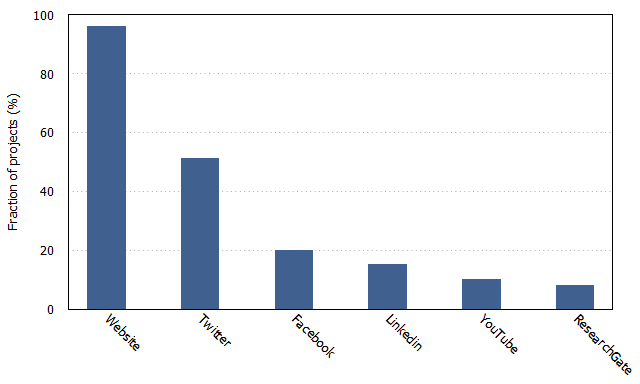
\includegraphics[scale=0.45]{Images/Social_media.png}
 \caption{Fractions of FET projects funded within the Horizon 2020 programme making use of the communication channels considered for this thesis.}
 \label{Social_media}
 \end{center}
\end{figure}

YouTube and Instagram are not common communication channels among FET projects. This is probably due to the difficulty of collecting content with high visual impact and suitable for drawing attention of disparate audiences on the project's activity. The difficulty arises from the fact that objectives and results of FET research are often very technical and not appropriate for image-based communication. In the case of YouTube, there is the additional complication of the resources needed for the production of high-quality videos.

ResearchGate is also characterised by a low usage rate. The result indicates that this social media is not seen as a suitable channel for large-scale communication activity. The reason could be the reachable audience, which is typically limited to researchers active in similar investigation fields.

\section{Online presence breakdown} \label{Online_presence_breakdown}
The analysis in section \ref{Overall_use_of_channels} was repeated for the projects in the groups outlined in section \ref{Data_set}: HPC, QT and the others. This enabled a comparison of how disparate classes of FET projects make use of online communication channels. The amount of projects in each group active on the considered channels is available in table \ref{Social_media_breakdown_table}. The results expressed as a percentage are shown in figure \ref{Social_media_breakdown}. 

\begin{figure}[!t] 
 \begin{center}
 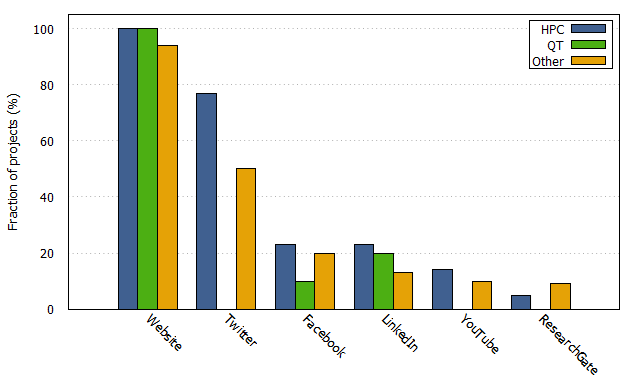
\includegraphics[scale=0.45]{Images/Social_media_breakdown.png}
 \caption{Fractions of FET projects funded within the Horizon 2020 programme making use of the communication channels considered for this thesis. Results are given as a function of three projects' groups: high-performing computing (HPC), quantum technologies (QT) and the other FET projects taken into account for the analysis. No QT project is active on Twitter, ResearchGate, YouTube or Instagram.}
 \label{Social_media_breakdown}
 \end{center}
\end{figure}

As already indicated by the results in section \ref{Overall_use_of_channels}, figure \ref{Social_media_breakdown} shows that basically all FET projects have created a website, regardless of the considered group. As for the most used social platforms within the FET community, i.e. Twitter, Facebook and Linkedin, the HPC class shows the largest fraction of opened accounts compared to QT and other projects. The result suggests that HPC projects have established one of the strongest online presences among FET initiatives.  

\begin{table}[t]
 \begin{center}
 {\footnotesize
  \begin{tabular}{cccc}
   \hline 
   \hline
   Channel & HPC & QT & Other \\ 
   \hline
   \hline
   Website & 22 & 10 & 92 \\
   Twitter & 17 & 0 & 50 \\
   Facebook & 5 & 1 & 21 \\
   LinkedIn & 5 & 1 & 21 \\
   ResearchGate & 1 & 0 & 9 \\
   YouTube & 3 & 0 & 6 \\
   Instagram & 1 & 0 & 2 \\
   \hline
   \hline
  \end{tabular}
 }
 \end{center} 
 \caption{Number of FET projects funded within Horizon 2020 making use of the communication channels considered for this thesis. Results are given as a function of the three projects' groups: high-performing computing (HPC, 22 projects), quantum technologies (QT, 10 projects) and the 98 other FET projects taken into account for the analysis.}
\label{Social_media_breakdown_table} 
\end{table}

The QT group seems to follow the opposite strategy. The fraction of projects making use of social media is significantly smaller compared to HPC and other FET projects. In particular, none of them has opened an account on Twitter, the most used social platform within the FET community. 

The limited use of social media made by QT projects highlights two facts. First, the QT Flagship will design its future online communication activity without guidelines based on previous experience from the same investigation field. Second, classes of projects facing similar challenges in terms of result communication and engagement of non-expert audiences may opt for very different strategies. This is the case of HPC and QT projects, which pursue very technical and often interconnected objectives, such as the common goal of improving current computers\footnote{Although both HPC and QT projects focus on the development of present-day computers, the strategies followed by the two groups are very different: the former aims at improving current classical architectures, the latter at exploiting a completely new approach based on the laws of quantum physics, see sections \ref{FET_and_high-performing_computing} and \ref{FET_and_quantum_technologies}.}.

\section{Budget impact} \label{Budget_impact}
The number of channels considered by the projects depends mainly on the pursued communication strategy and the available budget. The two factors are interconnected, as the latter impacts the former. Thus, it is worth assessing how deeply the online communication activity of FET projects is influenced by the allocated funding.  

\begin{figure}[!t] 
 \begin{center}
 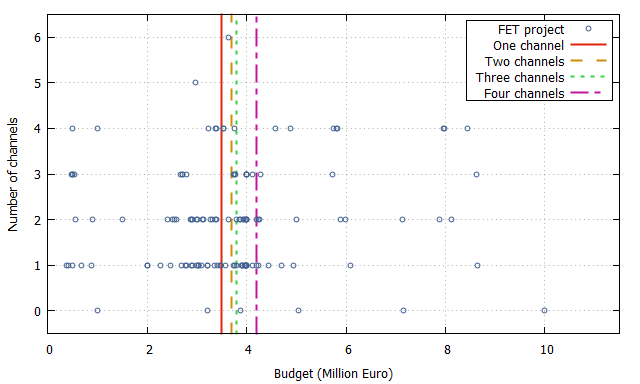
\includegraphics[scale=0.45]{Images/Channel_budget.png}
 \caption{Projects' distribution as a function of the available budget and of the number of considered online communication channels. The vertical lines are the budget medians of the groups of projects with one, two, three or four active channels. For the sake of clarity, the figure shows the budget range up to \euro 11.5 million. The following projects were used for the medians calculation but lie outside the plotted budget range:  DEEP-EST (\euro 15.9 million, three channels), FLAG-ERA II (\euro 18.3 million, two channels) and QuantERA (\euro 40.5 million, three channels).}
 \label{Channel_budget}
 \end{center}
\end{figure}

One approach in this direction consists of searching for the dependence of the number of channels on the available fund. To this aim, the following analysis was performed. First, projects were distributed on a plane as a function of the budget and of the number of channels, see figure \ref{Channel_budget}. As the plot shows, the majority of the projects has activated a number of channels between one and four. Hence, four groups of projects were considered, based on the amount of activated channels (from one to four). The other projects were disregarded for the analysis presented in this section due to their limited number. For each of the four groups, the median of the corresponding projects' budgets was calculated. The median was preferred to the arithmetic mean as it is a more robust indicator in the presence of outliers. The values are reported in table \ref{Median} and drawn as vertical lines in figure \ref{Channel_budget}. 

The analysis suggests a weak correlation between the number of active channels and the budget. On one hand, the larger the median, the higher the number of channels. On the other hand, the variation between the median values is typically of the order of percent. Moreover, it must be borne in mind the the data on the budget correspond to the total available funding, and not to the fraction allocated for communication purposes. Hence, in absolute terms of funding, and remembering that budgets are distributed over the project's duration (some years), the differences are not significantly large. The result indicates that the number of considered channels is not strongly influenced by the budget, but rather by the pursued communication strategy. 

\begin{table}[t]
 \begin{center}
  \begin{tabular}{cc}
   \hline 
   \hline
   Number of channels & Budget median \\ 
   \hline
   \hline
   One & 3.5 \\
   Two & 3.7 \\
   Three & 3.8 \\
   Four & 4.2 \\
   \hline
   \hline
  \end{tabular}
 \end{center} 
 \caption{Medians of the projects' budgets as a function of the number of channels considered by the projects. Values are rounded and expressed in million Euro.}
\label{Median} 
\end{table}

\section{Budget impact: the case of the HPC and QT projects} \label{Budget_impact_the_case_of_the_HPC_and_QT_projects}
The approach followed in section \ref{Budget_impact} enabled a further comparison of the communication strategies followed by HPC and QT projects. Figure \ref{Channel_budget_breakdown} shows the distribution of the projects in the two classes as a function of the budget and of the number of active channels. Typically, QT projects lie in the range between \euro 2 and \euro 4 million and have one active channel. HPC projects in the same budget window have typically considered more communication platforms. The result highlights the different communication strategy followed by the two classes of projects, as discussed in section \ref{Online_presence_breakdown}. 

\begin{figure}[!t] 
 \begin{center}
 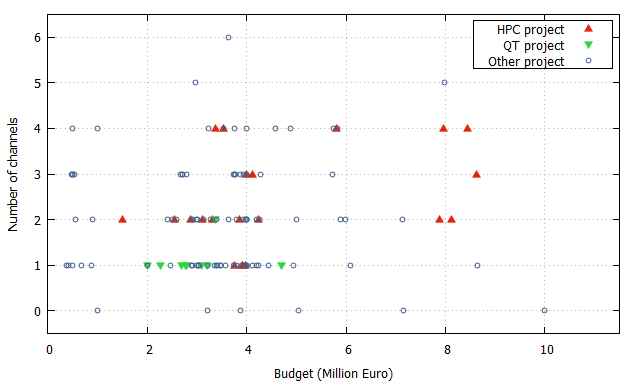
\includegraphics[scale=0.45]{Images/Channel_budget_breakdown.png}
 \caption{Distribution of HPC and QT projects as a function of the available budget and of the number of considered online communication channels. For the sake of clarity, the figure shows the budget range up to \euro 11.5 million. The QuantERA project (\euro 40.5 million, 3 channels) lies outside the plotted budget range.}
 \label{Channel_budget_breakdown}
 \end{center}
\end{figure}

\section{Chapter summary} 
In this chapter, the following items have been discussed:

\begin{enumerate}
 \item FET projects make use of disparate online communication channels. The most used channels are websites, Twitter and Facebook. Only a very limited fraction of projects is active on channels based on visual content such as YouTube and Instagram.
 \item The number of considered channels depends strongly on the class of FET project. HPC projects are among the most active initiatives. On the contrary QT project have very limited presence on the social platforms considered for this thesis.
 \item The available budget has a limited impact on the number of active channels. Thus, the amount of social platforms considered by the projects depends mainly on the pursued communication strategy.
 \item The indication in the previous point holds for the HPC and QT classes. An analysis of the projects within the same budget range shows that the two groups tend to follow opposite strategies. In general, HPC projects are present on several channels, whereas QT initiatives limit their online communication to the use of the website.       
\end{enumerate}